
\documentclass{article}


\usepackage{amsmath}
\usepackage{tikz}
\usepackage{float}
\usepackage{graphicx}
\usepackage{hyperref}

\usetikzlibrary{arrows}
\usetikzlibrary{positioning}

\begin{document}


\section{Experimental results and analysis}


\subsection{Experiments}

\subsubsection{Implementations}

We implement the algorithm on 3 POMDP problems: tiger and rock sample problem, which 
are discribed briefly as bellows:

\paragraph{Tiger problem:} There is 2 doors (left door and right door) for 
the agent to escape from the
room. However, there is only one door leading to the exit. There is a tiger 
behind the other door. The agent purpose is to open the door to exit, and 
to avoid the door containing the tiger. The agent can open the left door, 
open the right door, or to hear to the sound coming from the 2 doors. By 
hearing the sound, the agent can identify if the tiger is on the left door, 
or on the right door with the accuracy of 0.85. The cost for hearing action
is -1. The penalty for opening the door having the tiger is -100. The
reward for open the door to exit is +10.

The problem is modeled as 2 MDPs in \autoref{fig:TPTigerLeftMdl} and 
\autoref{fig:TPTigerRightMdl}.

\begin{figure}[H]
\centering

	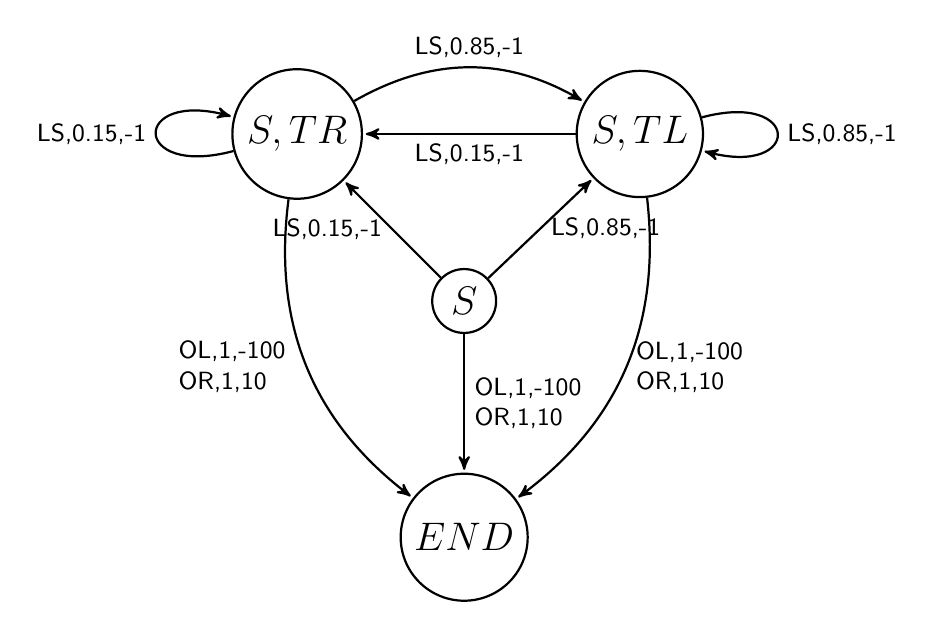
\begin{tikzpicture}[->,>=stealth',shorten >=1pt,auto,node distance=3cm,
	thick,main node/.style={circle,fill=white!20,draw,font=\sffamily\Large\bfseries}]

	\node[main node] (2) {$S,TR$};
	\node[main node] (1) [below right of=2] {$S$};
	\node[main node] (3) [right=2.7cm of 2] {$S,TL$};
	\node[main node] (4) [below of = 1] {$END$};

	\path[every node/.style={font=\sffamily\small}]
		(1) edge node [left] {LS,0.15,-1} (2)
			edge node [right] {LS,0.85,-1} (3)
			edge node [text width=1.5cm, align=left] {OL,1,-100\\OR,1,10} (4)
		(2) edge [loop left] node {LS,0.15,-1} (2)
			edge [bend left] node {LS,0.85,-1} (3)
			edge [bend right] node [text width=1.5cm, left] {OL,1,-100\\OR,1,10} (4)
		(3) edge [loop right] node {LS,0.85,-1} (3)
			edge node {LS,0.15,-1} (2)
			edge [bend left] node [text width=1.5cm, right] {OL,1,-100\\OR,1,10} (4);

	\end{tikzpicture}
	\caption{MDP Model for tiger on the left door}
	\label{fig:TPTigerLeftMdl}
\end{figure}

\begin{figure}[H]
\centering

	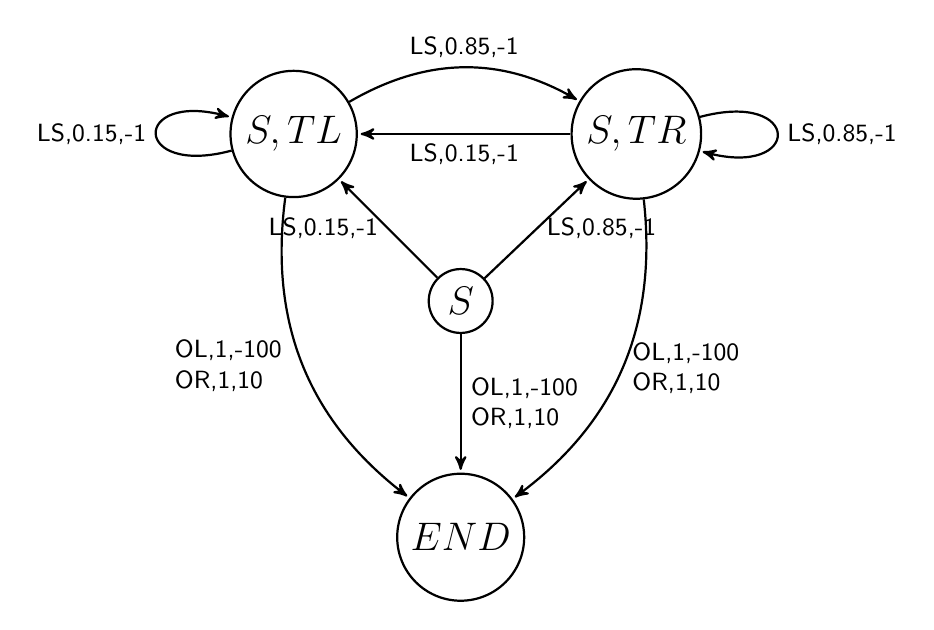
\begin{tikzpicture}[->,>=stealth',shorten >=1pt,auto,node distance=3cm,
	thick,main node/.style={circle,fill=white!20,draw,font=\sffamily\Large\bfseries}]

	\node[main node] (2) {$S,TL$};
	\node[main node] (1) [below right of=2] {$S$};
	\node[main node] (3) [right=2.7cm of 2] {$S,TR$};
	\node[main node] (4) [below of = 1] {$END$};

	\path[every node/.style={font=\sffamily\small}]
		(1) edge node [left] {LS,0.15,-1} (2)
			edge node [right] {LS,0.85,-1} (3)
			edge node [text width=1.5cm, align=left] {OL,1,-100\\OR,1,10} (4)
		(2) edge [loop left] node {LS,0.15,-1} (2)
			edge [bend left] node {LS,0.85,-1} (3)
			edge [bend right] node [text width=1.5cm, left] {OL,1,-100\\OR,1,10} (4)
		(3) edge [loop right] node {LS,0.85,-1} (3)
			edge node {LS,0.15,-1} (2)
			edge [bend left] node [text width=1.5cm, right] {OL,1,-100\\OR,1,10} (4);

	\end{tikzpicture}
	\caption{MDP Model for tiger on the right door}
	\label{fig:TPTigerRightMdl}
\end{figure}


\paragraph{Rock sample problem:} There is an environment represented by a 
grid of $m\times n$ cells, and an exit area on the right side of the grid. 
In this environment, there are $k$ rocks of type either good or bad. 
There is a rover at the starting position. The rover's task is to sample 
good rock and to move to the exit area. The position of $k$ rocks are known
to the rover, but the types of rocks is unknown. The rover is equipped with
a sensor to detect the type of rock with the accuracy of 
$0.5 + 0.5 \times 2^{-d/d_0}$, where $d$ is the distance from the rover to 
the checked rock, and $d_0$ is a constant. The rover can only sample a rock
at its position. If the rock is good, the rover receives reward of 10. If the 
rock is bad, the rover receives reward of -10. Apart from checking, and sampling, 
the rover can move north, east, west, south in the grid. There is high cost for 
moving out of the grid. Moving to exit areas yields reward of 10.

In our experiment, there are 7 rows and 8 columns. There are 8 rocks
locating at $\{(0,1), (1,1), (1,4), (1,6), (3,6), (4,3), (6,1), (6,5)\}$
(\autoref{fig:RSProb}).

\begin{figure}[h!]
\centering
\includegraphics[width=0.5\textwidth]{rocksample.png}
\caption{Rock Sample problem}
\label{fig:RSProb}
\end{figure}

In this problem, the probability of a rock is good (or bad) is independent from one
rock to another. Hence, instead of having a state as a tuple 
$(S_{x,y},R_{0,status}, R_{1,status}, \dots, R_{7,status})$, 
where $S_{x,y} \in \{s_{0,0}, s_{0,1}, \dots, s_{7,7}\}$ 
is the position of the rover, $R_{i,status} \in \{r_{i,bad}, r_{i,good}\}$,
$i=0,1,\dots,7$ are the rocks' status; we model each status as a tuple
$(S_{x,y},R_{i,status})$ (since each action of the rover can only
affect one rock status distribution at a one time). This reduces the computation
of the program. Hence, we directly model the mean MDP as bellows:

\begin{itemize}

\item Belief: $b(i), i=0,1,2,\dots,7$ is the probability of the 
i\textsuperscript{th} rock's status being good

\item States: $\{(S_{x,y},R_{i,status}), S_{x,y}\}$ (states with observation, and 
states without observation)

\item Actions: $\{north, east, west, south, sampling, check_i\}, i=0,1,2,\dots,7$ 
($check_i$ means checking the i\textsuperscript{th} rock's status)

\item Transition functions:
	\begin{itemize}
	\item Moving action (north, east, west, south) is deterministic and only changes
	the rover's position.\\ 
	E.g., $P( (S_{x+1,y},R_{0,good}) | (S_{x,y},R_{0,good}, south) ) = 1.0$,\\
	$P( S_{x+1,y} | S{x,y}, south) = 1.0$
	\item Samping action: $P( S_{x,y} | (S_{x,y}, R_{i,status}), sample) = 1.0$,\\
	$P( S_{x,y} | S_{x,y}, sample) = 1.0$
	\item Checking action:\\
    \begin{equation*}
    	\begin{aligned}
	P( (S_{x,y}, R_{i,good}) &| (S_{x,y}, R_{j,status}, check_i) ) \\
		&= \alpha \\
		&= b(i)acc(S_{x,y}, i) + (1 - b(i))(1 - acc(S_{x,y}))
		\end{aligned}
    \end{equation*}
    where, $acc(S_{x,y},i)$ is the accuracy 
	of sensor given the rover at $(x,y)$ and checking the i\textsuperscript{th} rock.
	\begin{equation*}
		P( (S_{x,y}, R_{i,bad}) | (S_{x,y}, R_{j,status}, check_i) ) = 1 - \alpha
	\end{equation*}
	\end{itemize}

\item Reward functions: Only action sampling and moving resulting in rewards as bellows.
	\begin{itemize}
	\item Moving action (deterministic): If the rover goes to exit area, it receives a 
	reward of 10. If the rover goes out of the grid (not exit area), it receives a
	penalty of -1000.
	\item Sampling action: $R(S_{x,y}, sample) = 10 \times b(i) - 10 \times (1 - b(i))$,
	where $i$ is the index of the sampled rock.
	\end{itemize}

\end{itemize}

\paragraph{Notes:} There is an end state for the agent moving to exit area. In 
end state, the agent can only move into end state under any action. The reward is
zero for any action taken in end state.

\subsubsection{Experiment Setup and Results}

\paragraph{Tiger problem:} The game is just one episode, which means that the game is over
when you open the door. We run 5000 simulations for this games. The experimental parameters
are as follows:
\begin{itemize}
\item Discount factor: 0.95
\item Simulation length: 5000
\end{itemize}

The results are in \autoref{tab:TP1Eps}

\begin{table}[H] 
\begin{center}
	\begin{tabular} {| c | c | c |}
	\hline \hline
	Tuned Dis-RB & Belief to Open door & Expected return \\
	\hline
	0.007 & [0.9698,0.0302] & 3.476 \\
	\hline
	0.01 & [0.9945,0.0055] & 3.821 \\
	\hline
	0.07 & [0.999,0.001] & 2.674 \\
	\hline \hline
	\end{tabular}
\end{center}
\caption{Tiger Problem for one episode}
\label{tab:TP1Eps}
\end{table}

For POMDP algorithm, they assume that the game can be restarted after opening action taken, 
which means there are infinite number of episodes. Hence, we do another experiment with 
100 episodes to compare with POMDP algorithm. After 100 episodes, the discount factor is
negligible, so we could take 100 episodes as an approximation to infinite number of episodes.
The experimental parameters are as bellows:
\begin{itemize}
\item Discount factor: 0.95
\item Simulation length: 500
\item Number of episodes in each game: 100
\end{itemize}

The results are in \autoref{tab:TPINFEps}

\begin{table}[H] 
\begin{center}
	\begin{tabular} {| c | c | c |}
	\hline \hline
	Tuned dis-RB & Belief to Open door & Expected return \\
	\hline
	0.007 & [0.9698,0.0302] & 18.953 \\
	\hline
	0.01 & [0.9945,0.0055] & 16.303 \\
	\hline 
	0.07 & [0.999,0.001] & 9.097 \\
	\hline \hline
	\end{tabular}
\end{center}
\caption{Tiger Problem for infinite episode game}
\label{tab:TPINFEps}
\end{table}


\paragraph{Rock sample problem:} In order to compare with other online POMDP algorithms,
we add a discount factor to our algorithm. We set our discount factor the same as their 
$discount_{factor}=0.95$. The experimental paramters are as follows:
\begin{itemize}
\item $discount_{factor}=0.95$
\item $d_0=20$
\item The world model is described in \autoref{fig:RSProb}.
\end{itemize}

We set $the discount-RB=0.0001$ in this experiment. We run the simulation for each starting rock
configuration 10 times (i.e., 10 runs for each of the $2^8$ different joint rock types). The
initial belief state is the same for all these runs (probability each rock is good is 0.5).

The result is shown in the \autoref{tab:RSCompareOtherAlg}

\begin{table}[H]
\begin{center}
	\begin{tabular} {| l | c | c |}
		\hline \hline
		Algorithm & Return & Computation time (ms) \\
		\hline
		AEMSI (using Bline policy as lower bound) & 7.35 & 900 \\
		\hline
		HSVI-BFS (using Blind policy as lower bound) & 20.75 & 859 \\
		\hline
		AEMSI (using PBVI as a lower bound) & 17.1 & 954 \\
		\hline
		HSVI-BFS (using PBVI as a lower bound) & 21.46 & 826 \\
		\hline
		Our algorithm (no pre-computed lower bound) & 18.7 & 300 \\
		\hline \hline
	\end{tabular}
\end{center}
\caption{Rock sample results compared with other online algorithms}
\label{tab:RSCompareOtherAlg}
\end{table}

To know whether the distribution of rocks affects the final return. We set up a different
experiment with different rocks distribution as in \autoref{fig:RSDiffEnvir}

\begin{figure}[H]
\centering
\includegraphics[width=0.8\textwidth]{Diff-Envir-Rock-Sample.png}
\caption{Different environment setup}
\label{fig:RSDiffEnvir}
\end{figure}

The results are shown in the \autoref{tab:RSDiffEnvir}

\begin{table}[H]
\begin{center}
	\begin{tabular} {| c | c | c |}
		\hline \hline
		Algorithm & Return & Computation time (ms) \\
		\hline
		Our algorithm (no pre-computed lower bound) & 20.3 & 300 \\
		\hline \hline
	\end{tabular}
\end{center}
\caption{Results in another environment setup}
\label{tab:RSDiffEnvir}
\end{table}


\subsection{Analysis}

\subsubsection{Tiger problem:} 
In the case of one-episode game \autoref{tab:TP1Eps}, we can see that the highest 
expected reward is 3.821, and its
corresponding belief to open the door is [0.9945,0.0055]. This belief is different from
the policy computed by standard POMDP algorithm, which suggests we should open the door
when the belief reaches [0.9698,0.0302]. The difference lies in the setup of POMDP algorithm 
for tiger problem. The policy computed by POMDP algorithm is for infinite episodes (the game
can be restarted). Hence, compared with 1-episode game, the optimal policy is to choose
opening action sooner as the agent can receive future reward in future episodes.

In the case of infinite-episode game \autoref{tab:TPINFEps}, we can see that the optimal belief
to open the door is [0.9698,0.0302], which is exactly the same with the policy computed by POMDP
algorithm.

\subsubsection{Rock sample problem:} 
In \autoref{tab:RSCompareOtherAlg}, we can see that
the running time of our algorithm is significantly less than other online algorithms,
and we do not need any pre-computed lower bound or upper bound. The reason for our final
return is smaller than HSVI is that our reward has been discounted a lot, which means the
agent spends more steps moving around before sampling. It is explained by the reward bonus
for checking action can overwhelm the reward for sampling action. Hence, this problem is
controlled by the reward bonus discount factor.

In \autoref{tab:RSDiffEnvir}, we see that the agent get higher reward in this environment 
setup because the agent samples most of the good rocks on its way out. This means it does
not need to go back sample some rocks,so the reward is discounted less.

In brief, our algorithm performs well on rock sample problem. It computes the policy fast,
which meets the requirement of online tasks. If there is a discount factor, the total 
discounted reward it gets is slightly less than HSVI and the return depends on the rock 
distribution.

\subsubsection{Comparison with BEB \cite{kolter} and Variance-based approach \cite{sorg}:}

The BEB approach \cite{kolter} and our algorithm are based on different problem setup: the BEB
assumes the transition functions are modeled as Dirichlet distributions, while in our problem, the 
belief of MDPs is modeled as discrete distribution. However, if we only consider the reward
bonus formula, there is a crucial difference between the two approaches. In BEB approach, 
reward bonus for every state-action pair is treated the same way (only depends on the number
of state-action pair visits). Hence, they implicitly assume that the information they get
is proportional to the number of state-action pair visits. However, it is more precise that
the information we get for visiting a state-action pair depends on the change in belief
after executing that state-action pair, which is the intuition behind our reward bonus formula.
For example, in tiger problem, the reward bonus for both listening and opening action are in
similar relationship with number of taking these actions (since there is only 1 state). Hence,
the agent could take the opening action too early due to the reward bonus, which results in
non-optimal policy. The same consequence can happen to rock sample problem with sampling action.

Talking about the Variance-based approach \cite{sorg}, as the reward bonus depends on the variance of the
transition functions and reward functions over the belief, the reward bonus is assigned a
non-zero value as long as the belief is uncertain. For example, in the case of tiger
problem, the reward bonus for open action will be non-zero. This could be dangerous and result
in non-optimal policy because the reward bonus could encourage the agent to take opening action
when the belief is highly uncertain. The same consequence can happen to rock sample problem,
which is the reward bonus encourages the agent to take sampling action, even though the belief
is uncertain.

\section{Conclusions and future work}

In this report, we come up with a better-running-time algorithm for solving POMDP problem in which unobservable states are discrete and static. The main idea is 
to covert the POMDP into a finite number of MDPs, and to apply reinforcement learning
approach with reward bonus on the mean MDP of these MDPs over the belief.

We prove theoretical bound for the algorithm as in \cite{kolter}, that our algorithm only
performs suboptimally in a polynomial number of steps. We also apply our algorithm to solve
problems of Tiger and Rock Sample. The experimental results show a better running time 
compared with other online POMDP algorithms.

\paragraph{} In brief, our algorithm has advatanges and disadvantages as bellows:
\begin{itemize}
\item Advantages: Our algorithm gives better running time compared with
other online POMDP algorithms.
\item Disadvantages: There are two main disadvantages of our algorithm: (1)
it can only be applied to a limited domain of POMDP problem of discrete and 
static unobservable states; (2) to obtain good policy, our algorithm requires
to tune the value of reward bonus discount.
\end{itemize}

\paragraph{} In the future, it is interesting to investigate how to handle the dynamic environment, and how to choose reward bonus discount so that we get better policy.


\begin{thebibliography}{9}

\bibitem{smith}
	T Smith, R Simmons. \emph{Heuristic search value iteration for POMDPs} - Proceedings of the 20\textsuperscript{th} conference on Uncertainty in AI, 2004.

\bibitem{kurn}
	H Kurniawati, D Hsu, WS Lee. \emph{SARSOP: Efficient Point-Based POMDP Planning by Approximating Optimally Reachable Belief Spaces} - Robotics: Science and Systems, 2008.

\bibitem{kolter}
	Z Kolter and A Y Ng. \emph{Near-bayesian exploration in polynomial time} - In Proceedings to International Conference on Machine Learning, 2009.

\bibitem{sorg}
	Sorg, S Singh, and RL Lewis. \emph{Variance-based rewards for approximate Bayesian reinforcement learning} - In Proceedings to Uncertainty in AI, 2010.

\bibitem{ross}
	S Rosss, J Pineau, S Chaib-Draa. \emph{Online Planning Algorithm for POMDPs}. J. Artif.
	Intelligence, 2008.

\end{thebibliography}

\end{document}
